\documentclass[a4paper, 12pt]{article}

% Useful packages
\usepackage[utf8]{inputenc} % for handling accents
\usepackage{amsmath} % for advanced math
\usepackage{graphicx} % for handling images
\usepackage[hidelinks]{hyperref} % for hyperlinks
\usepackage{geometry} % for margin settings
\usepackage{xcolor} % for custom colors
\usepackage{titlesec} % for customizing section titles
\usepackage{titling} % for custom title, subtitle, and organization
\usepackage{algorithm} % for pseudocode
\usepackage{algorithmicx}
\usepackage{algpseudocode} % for pseudocode
\usepackage{amsfonts}
\usepackage{float} % for H float specifier

% Margin settings
\geometry{a4paper, margin=1.8cm}

% Define custom colors
\definecolor{sectioncolor}{RGB}{0, 51, 102} % darker blue
\definecolor{subsectioncolor}{RGB}{0, 102, 102} % darker teal

% Customize section, subsection, and subsubsection without numbers
\titleformat{\section}
  {\color{sectioncolor}\large\bfseries} % Color and size for \section
  {}{0em}{} % Remove section number

\titleformat{\subsection}
  {\color{subsectioncolor}\normalsize\bfseries} % Color and size for \subsection
  {}{0em}{} % Remove subsection number

\titleformat{\subsubsection}
  {\color{subsectioncolor}\small\bfseries} % Color and size for \subsubsection
  {}{0em}{} % Remove subsubsection number

\begin{document}
\begin{titlepage}
    \centering
    \vspace*{\fill}
    {\LARGE \textbf{UNIVERSITY OF PISA}}\\[0.5cm]
    \begin{figure}[h]
        \centering
        
\includegraphics[width=0.4\textwidth]{media/universita-di-pisa-logo.png} 
    \end{figure}
    {\Large \textit{Artificial Intelligence and Data Engineering}}\\[1.5cm]
    {\LARGE \textbf{Cloud Computing}}\\[1cm]
    {\Large \textit{Hadoop Letter Frequency}}\\[8cm]
    {\large \textbf{Authors: Gemelli M. Namaki D. Nocella F.}}\\[0.5cm]
    {\large Academic Year 2023/2024}
    \vspace*{\fill}
\end{titlepage}


\tableofcontents
\newpage
\section{Introduction}
The objective of this project is to implement a data processing pipeline that can handle substantial data sets, ensuring efficient computation and meaningful data insights. By exploiting the MapReduce paradigm, data processing tasks is split into two main functions: the \textbf{Mapper} and the \textbf{Reducer}.\newline
The Mapper function processes and filters the input data, emitting \textbf{key-value pairs}, while the Reducer function aggregates and processes these pairs to produce the final output.\\

\noindent The project was developed using the Hadoop framework, which provides an open-source implementation of the MapReduce paradigm. Hadoop allows for the distributed processing of large data sets across clusters of computers using simple programming models. The Hadoop ecosystem also includes other tools, such as HDFS (Hadoop Distributed File System) for distributed storage, and YARN (Yet Another Resource Negotiator) for cluster resource management.\newline

\noindent Given a text document as input, it is aimed to extract the frequency of each letter composing such document. In Order to achieve this, two differnt jobs are required: the first job is responsible for counting the number of letters in the document, while the second job is responsible for evaluating the frequency of each letter. Finally, the results obtained from the processing pipeline will be shown.



\section{Algorithm Design}
The objective of this project is to analyze letter frequency in text documents utilizing Hadoop's MapReduce framework. Specifically, two distinct approaches were implemented to optimize the MapReduce task: the use of a Combiner and the implementation of an In-Mapper Combiner. These methods aim to enhance the efficiency of the MapReduce process by reducing the amount of data transferred between the Mapper and Reducer stages.

\subsection{MapReduce with Combiner}
The Combiner is a mini-reducer that processes the output of the Mapper tasks before passing it to the Reducer. By aggregating the intermediate data locally on the mapper nodes, the Combiner reduces the volume of data shuffled across the network, thus improving the performance of the MapReduce job. It performs its operations on the same node where the mapper is running.
\subsubsection{Pseudocode}
\begin{algorithm}[H]
    \caption{Letter Count with Combiner}
    \begin{algorithmic}[1]
        \Require Txt file
        \Ensure Total count of each letter in the input file
        
        \vspace{1em}
        \Statex
        \noindent \textbf{Mapper}
        \Procedure{Setup}{context}
        \State normalize $\leftarrow$ context.getConfiguration().get("normalize")
        \EndProcedure

        \Procedure{Map}{Object key, Text value}
        \State line $\leftarrow$ Normalize(value.toString(), normalize) \Comment{Remove accents and set lowercase}
        \For{each character $c$ in line}
        \State EmitIntermediate(LETTER\_COUNT\_KEY, 1)
        \EndFor
        \EndProcedure

        \vspace{1em}

        \Statex
        \noindent \textbf{Combiner \& Reducer}
        \Procedure{Reduce}{Text key, Iterable$<$LongWritable$>$ values}
        \State sum $\leftarrow$ 0
        \For{each LongWritable val in values}
        \State sum $\leftarrow$ sum + val.get()
        \EndFor
        \State Emit(key, new LongWritable(sum))
        \EndProcedure
    \end{algorithmic}
\end{algorithm}



\begin{algorithm}[H]
    \caption{Letter Frequency with Combiner}
    \begin{algorithmic}[1]
        \Require Txt file, Total number of characters in the txt file
        \Ensure Frequency of each letter in the input file

        \Statex
        \noindent \textbf{Mapper}
        \Procedure{Setup}{context}
        \State normalize $\leftarrow$ context.getConfiguration().get("normalize")
        \EndProcedure

        \Procedure{Map}{Object key, Text value}
        \State line $\leftarrow$ Normalize(value.toString(), normalize) \Comment{Remove accents and set lowercase}
        \For{each character $c$ in line}
        \State EmitIntermediate(String.valueOf($c$), 1)
        \EndFor
        \EndProcedure

        \vspace{1em}

        \Statex
        \noindent \textbf{Combiner}
        \Procedure{Reduce}{Text key, Iterable$<$LongWritable$>$ values}
        \State sum $\leftarrow$ 0
        \For{each LongWritable val in values}
        \State sum $\leftarrow$ sum + val.get()
        \EndFor
        \State Emit(key, new LongWritable(sum))
        \EndProcedure

        \vspace{1em}

        \Statex
        \noindent \textbf{Reducer}
        \Procedure{Setup}{context}
        \State letterCount $\leftarrow$ context.getConfiguration().getLong("letterCountValue", 1)
        \EndProcedure

        \Procedure{Reduce}{Text key, Iterable$<$LongWritable$>$ values}
        \State sum $\leftarrow$ 0
        \For{each LongWritable val in values}
        \State sum $\leftarrow$ sum + val.get()
        \EndFor
        \State freq $\leftarrow$ (double) sum / (double) letterCount
        \State Emit(key, new DoubleWritable(freq))
        \EndProcedure
    \end{algorithmic}
\end{algorithm}

\subsection{MapReduce with In-Mapper Combiner}
The In-Mapper Combiner combines the mapping and combining steps within the Mapper itself. This method involves accumulating the results in a data structure within the Mapper, which is then emitted at the end of the mapping phase. This approach minimizes the overhead of multiple data passes by efficiently combining intermediate results within the Mapper, reducing the need for external Combiner steps and further optimizing network usage and processing time.
\subsubsection{Pseudocode}
\begin{algorithm}[H]
    \caption{Letter Count with In-Mapper Combiner}
    \begin{algorithmic}[1]
    \Require Txt file
    \Ensure Total count of each letter in the input file
    
    \vspace{1em}

    \Statex
    \noindent \textbf{Mapper}
        
        \Procedure{Setup}{Context context}

            \State normalize $\leftarrow$ context.getConfiguration().get("normalize")

            \State map $\leftarrow$ \{\}

            \State letterCountKey $\leftarrow$ new Text("total\_letter\_count")

        \EndProcedure
    
        \vspace{1em}

        \Procedure{Map}{Object key, Text value}
            \State line $\leftarrow$ Normalize(value.toString(), normalize)
            \For{each character $c$ in line}
                \State map\{{$letterCountKey$}\} $\leftarrow$ map\{{$letterCountKey$}\} + 1
            \EndFor
        \EndProcedure
    
        \vspace{1em}

        \Procedure{Cleanup}{Context context}
            \For{each entry $<k, v>$ in $map$}
                \State Emit($k$, $v$) \Comment {Emint key and count map\{key\}}
            \EndFor
        \EndProcedure
    
        \vspace{1em}

    \Statex
    \noindent \textbf{Reducer}

    
        \Procedure{Reduce}{Text key, Iterable$<$LongWritable$>$ values}
            \State sum $\leftarrow$ 0
            \For{each value in values}
                \State sum $\leftarrow$ sum + value
            \EndFor
            \State Emit(key, new LongWritable(sum))
        \EndProcedure

    \end{algorithmic}
    \end{algorithm}
    
    \begin{algorithm}[H]
    \caption{Letter Frequency with In-Mapper Combiner}
    \begin{algorithmic}[1]
    \Require Txt file, Total number of characters in the txt file
    \Ensure Frequency of each letter in the input file
    
    \vspace{1em}

    \Statex
    \noindent \textbf{Mapper}
        
        \Procedure{Setup}{Context context}
            \State normalize $\leftarrow$ context.getConfiguration().get("normalize")
        
        \State map $\leftarrow$ \{\}
        
        \EndProcedure

        \vspace{1em}

        \Procedure{Map}{Object key, Text value}
            \State line $\leftarrow$ Normalize(value.toString(), normalize)
            \For{each character $c$ in line}
                \State map\{$c$\} $\leftarrow$ map\{$c$\} + 1
            
            \EndFor
        \EndProcedure

        \vspace{1em}

        \Procedure{Cleanup}{Context context}
            \For{each entry $<k, v>$ in $map$} \Comment {Emit key and count map\{key\}}
                \State Emit($k$, $v$)
            \EndFor
        \EndProcedure
    
        \vspace{1em}

    \Statex
    \noindent \textbf{Reducer}
        
        \Procedure{Setup}{Context context}
            \State letterCount $\leftarrow$ context.getConfiguration().getLong("letterCountValue", 1)
        \EndProcedure

        \vspace{1em}

        \Procedure{Reduce}{Text key, Iterable$<$LongWritable$>$ values}
            \State sum $\leftarrow$ 0
            \For{each value in values}
                \State sum $\leftarrow$ sum + value
            \EndFor
            \State freq $\leftarrow$ (double) sum / (double) \textbf{letterCount}
            \State Emit(key, new DoubleWritable(freq))
        \EndProcedure

    \end{algorithmic}
    \end{algorithm}
    


\section{Results}

\subsection{Experimental Setup}
Executing the MapReduce workflow with different inputs, and configurations:
\begin{itemize}
  \item \textbf{Input size}: the size of the input file is varied to evaluate the performance of the MapReduce workflow.
        \begin{itemize}
          \item \textbf{Paradise Lost} $\sim$ 310 kb
          \item \textbf{Moby Dick} $\sim$ 421kb
          \item \textbf{Frankenstein} $\sim$ 440 kb
          \item \textbf{Divina Commedia} $\sim$ 600 kb
          \item \textbf{Gerusalemme Liberata} $\sim$ 691 kb
          \item \textbf{Promessi Sposi} $\sim$ 1.440 kb
          \item \textbf{Test file} (random generated sequence of char) of $\sim$ 800 Mb.
        \end{itemize}
  \item \textbf{Number of mappers}: Hadoop handles this step
  \item \textbf{Number of reducers}: From one up to three reducers are used for letter frequency
\end{itemize}

\subsection{Performance Evaluation}


\begin{figure}[ht!]
  \centering
  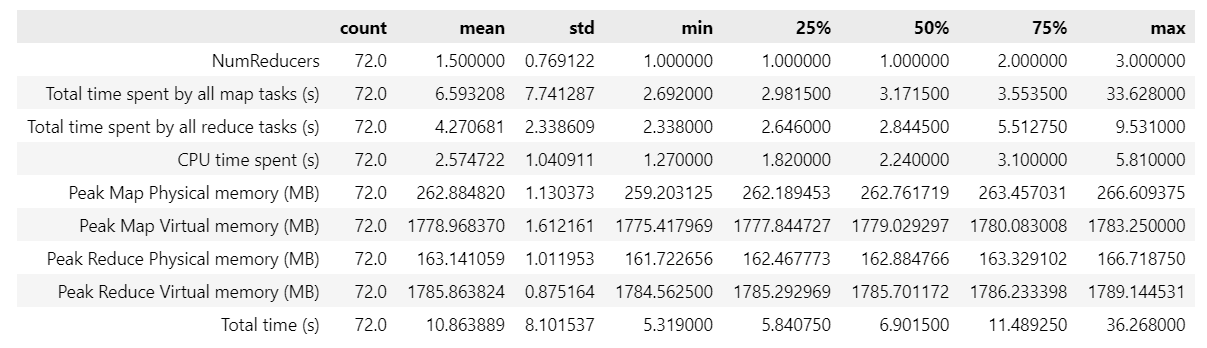
\includegraphics[width=\textwidth]{media/performance/opera_df_describe.png}
  \caption{Statics' insights on Operas}
  \label{fig:OperaInsights}
\end{figure}

\begin{figure}[ht!]
  \centering
  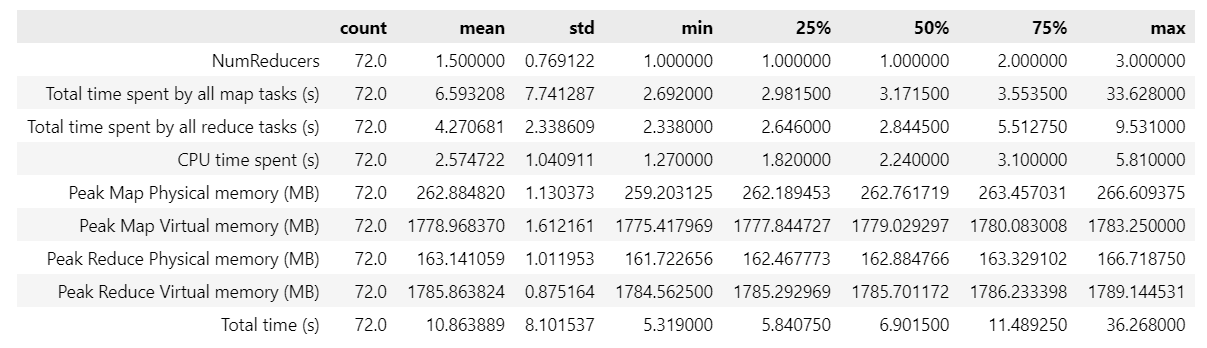
\includegraphics[width=\textwidth]{media/performance/opera_df_describe.png}
  \caption{Statics' insights on Test}
  \label{fig:OperaInsightsTEST}
\end{figure}


\begin{figure}[ht!]
  \centering
  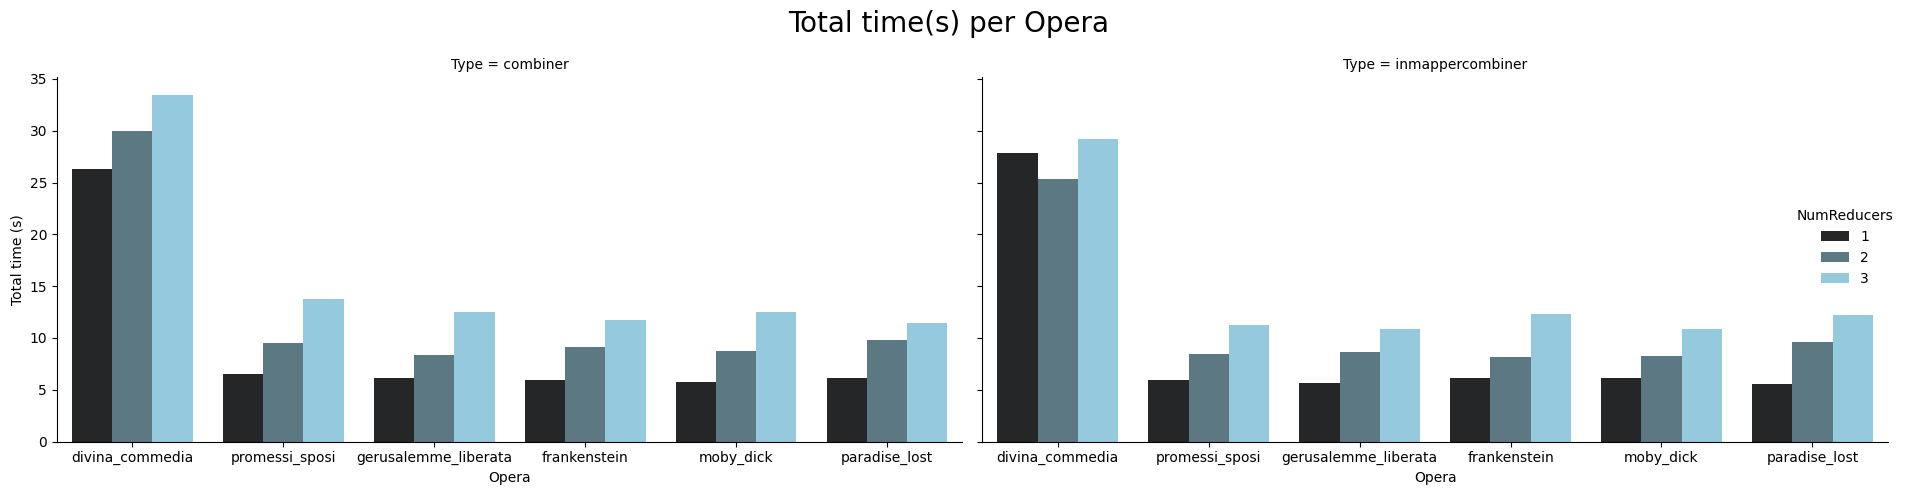
\includegraphics[width=0.8\textwidth]{media/performance/total_time_S_per_opera.png}
  \caption{Total time for each opera with different reducers}
  \label{fig:TimeOperas}
\end{figure}

\begin{figure}[ht!]
  \centering
  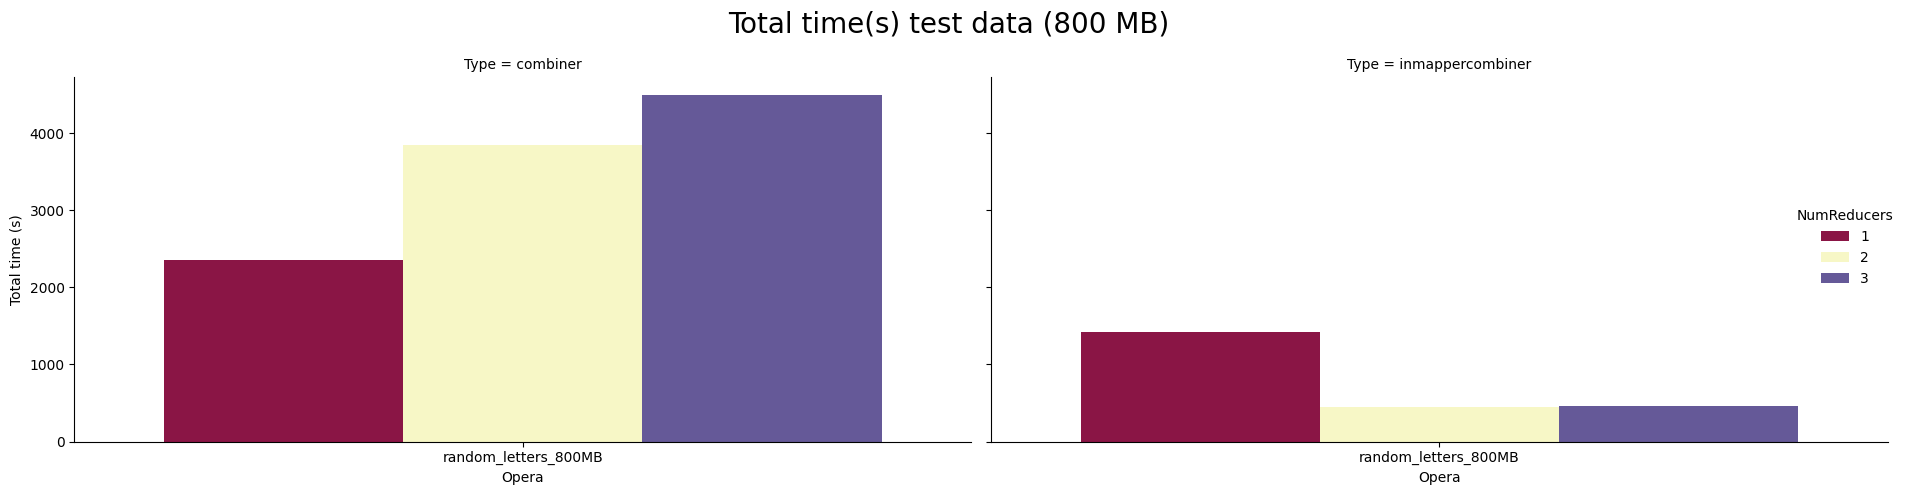
\includegraphics[width=0.8\textwidth]{media/performance/total_time_S_per_opera(TEST).png}
  \caption{Total time for Test with different reducers}
  \label{fig:TimeTest}
\end{figure}

\begin{figure}[ht!]
  \centering
  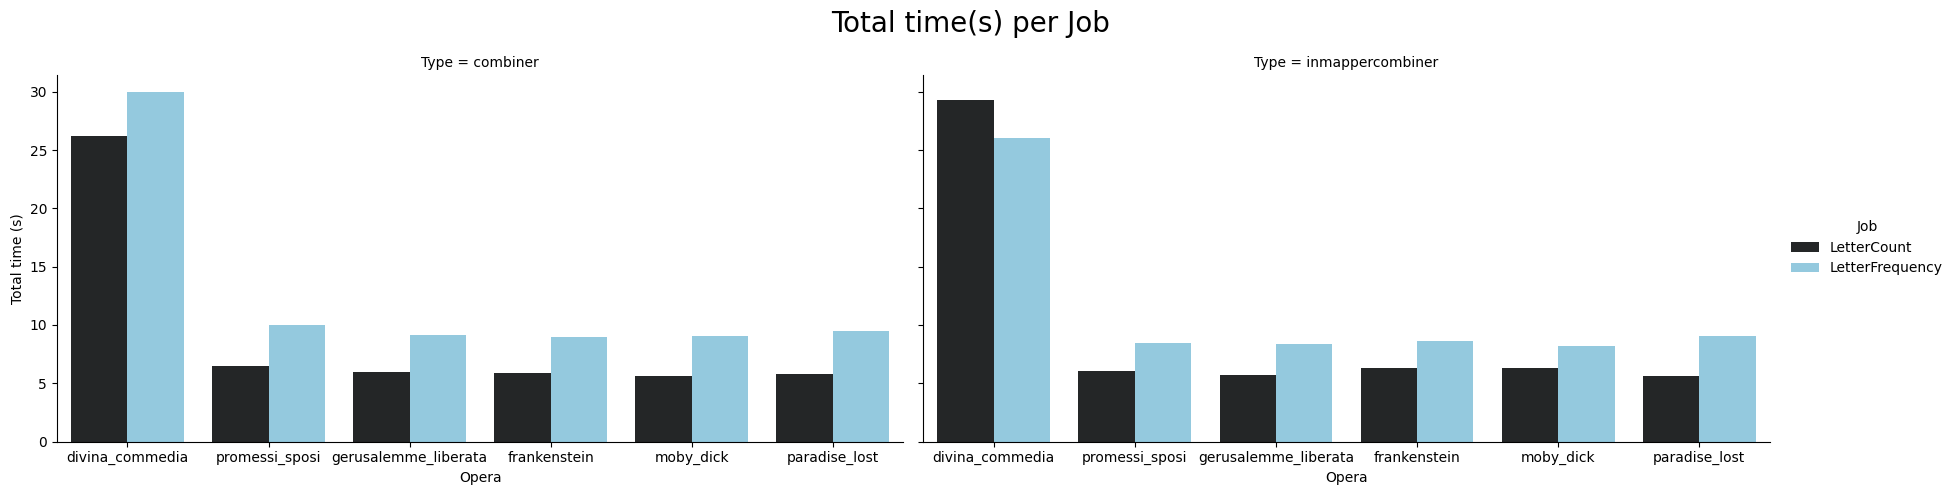
\includegraphics[width=0.8\textwidth]{media/performance/total_time_S_per_job.png}
  \caption{Total time for each job with different operas}
  \label{fig:TimeJob}
\end{figure}

\begin{figure}[ht!]
  \centering
  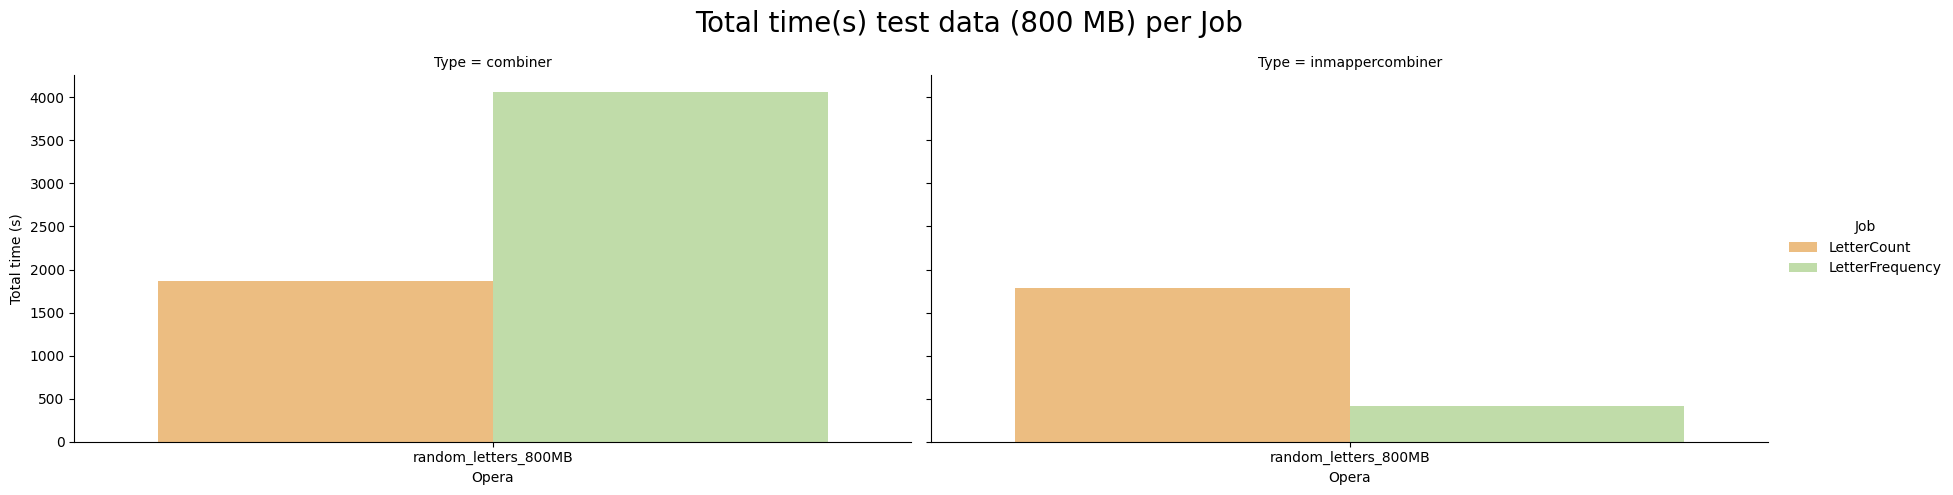
\includegraphics[width=0.8\textwidth]{media/performance/total_time_S_per_job(TEST).png}
  \caption{Total time for each job with Test}
  \label{fig:TimeJobTest}
\end{figure}

\section{Conclusions}



\end{document}
